\section{Durchführung}
\subsection{Fourier-Analyse}

Bei diesem Teil des Versuches sollen die Amplituden der einzelnen Oberwellen von
drei verschiedenen Spannungen bestimmt werden. Diese drei Spannungen sind eine
Rechteckspannung, eine Dreieckspannung und eine Sägezahnspannung. \\\\

Diese verschiedenen Spannungen werden von einem Funktionsgenerator erzeugt. Die
erzeugte Spannung wird auf ein Oszilloskop übertragen, in dem ein Analog-Digital-Konverter
und ein Rechner für eine Fourier-Transformation verbaut sind. Damit lässt sich die Spannung
und das Frequenzsprektrum gleichzeitig auf dem Oszilloskop anzeigen.

Der Analog-Digital-Konverter besitzt eine sogenannte Abtastfrequenz, da er nur in
endlichen Abständen die Spannung messen kann. Aus diesem Grund muss die Frequenz
der Spannung viel kleiner sein als die Abtastfrequenz. Es muss viel kleiner sein, da
diese Vorraussetzung auch für die Frequenzen der zu messenden Oberwellen gelten muss,
die eine größere Frequenz als die Spannung haben.
Bei den verwendeten Apparaturen sind diese Vorraussetzungen allerdings immer gegeben
und müssen bei der Durchführung nicht berücksichtigt werden.

Nun werden die einzelnen Amplituden der Oberwellen auf dem Oszilloskop dargestellt
und können mithilfe von dem Cursor abgelesen werden.

\subsection{Fourier-Synthese}

Der zweite Teil des Versuches besteht daraus, dass aus einzelnen Oberwellen die
drei oben genannten Spannungen zusammengesetzt werden sollen. Dazu müssen vorher
die Koeffizienten $a_n$ und $b_n$ für die verschiedenen Schwingungen theoretisch
bestimmt werden. Die Rechnungen dazu sind in der Auswertung angegeben.

Es wird ein Signalgenerator, der Sinusschwingungen erzeugt, für diesen Teil verwendet.
Der Generator kann bis zu 9 Sinusschwingungen, mit verschiedenen Amplituden und Phasen
erzeugen.

Als erstes müssen die verschiedenen Sinusschwingungen in Phase gebracht werden. Dazu
wird immer die erste Spannung und der Reihe nach die folgenden Spannungen auf
dem Oszilloskop, im XY-Betrieb, dargestellt. Auf dem Oszilloskop lassen sich nun
Lissajous-Figuren beobachten, die in Abhängigkeit von der Phasenverschiebung
anders aussehen. In Abbildung (\ref{fig:2}) sind zwei Beispiele gezeigt.
Mithilfe der Lissajous-Figuren, werden die einzelnen Sinusspannungen in Phase gebracht.
Besteht die zusammengesetzte Schwingung aus Cosinusschwingungen ist zu beachten,
dass $\sin\left(x + \frac{\pi}{2}\right) = \cos(x)$ gilt.

\begin{figure}[H]
  \centering
  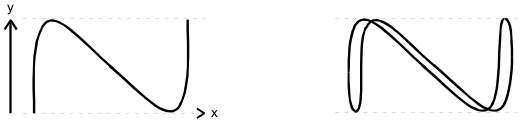
\includegraphics{Durchfuerung1.png}
  \caption{Lissajous-Figuren von zwei Cosinusschwingungen mit dem Frequenzverhältnis 1:3, links
  Phase $\phi=0$, rechts Phase $0<\phi<\frac{\pi}{2}$ [1].}
  \label{fig:2}
\end{figure}

Nun müssen noch die Amplituden der einzelnen Sinusschwingungen jeweils für die
darzustellende Spannung eingestellt werden. Die Amplituden werden mit einem
Millivoltmeter bestimmt. Es wird die Amplitude von der ersten Spannung ermittelt
und die anderen Spannungen werden, im Verhältnis zur ersten Spannung so eingestellt,
wie es in der theoretischen Rechnung für die jeweiligen Spannungen ermittelt wurde.

Zum Schluss werden die korrekt eingestellten Sinusspannungen durch den Ausgang
für die Summenschwingung auf dem Oszilloskop sichtbar gemacht. Es werden nach und
nach mehr Spannungen hinzugeschalt und bei jeder zugeschalteten Spannung wird ein
Thermodruck angefertigt.
